\documentclass[a4paper,12pt]{article}
\usepackage{graphicx}
\usepackage{bm,amssymb}
\usepackage{mathrsfs}
\usepackage[unicode,colorlinks=true,filecolor=blue, menucolor=black, linkcolor=black, citecolor=black,pagebackref=white]{hyperref}
\usepackage[utf8]{inputenc}
\usepackage[russian]{babel}
\usepackage{amsmath}
\usepackage{feynmp}
\usepackage{caption}
\usepackage[left=2cm,right=2cm, top=2cm,bottom=2cm,bindingoffset=0cm]{geometry}
\begin{document}
\title{Семинар по теме: метод перевала}
\maketitle

\section*{Ликбез}
Рассмотрим важный класс интегралов вида
\begin{equation} \label{eq:lec3:I}
I = \int\limits_{-\infty}^\infty e^{f(t)} dt,
\end{equation}
где $f(t)$ имеет \emph{резкий} (условие резкости обсудим чуть позже) максимум при $t=t_0$.

\noindent
Вблизи $t_0$:
\begin{equation} 
\label{eq:lec3:fTaylor}
f(t) \approx f(t_0) + \frac{f''(t_0)}2 (t-t_0)^2,\qquad f''(t_0) <0.
\end{equation}
Подставив это разложение в экспоненту, получаем гауссов интеграл, который элементарно вычисляется:
\begin{equation} \label{eq:lec3:Isaddle}
\boxed{I \approx
	%\int\limits_{-\infty}^\infty e^{f(x_0) + \frac{f''(x_0)}2 (x-x_0)^2} dx  =
	\sqrt{ \frac{2\pi}{|f''(t_0)|} } \; e^{f(t_0)} }
\end{equation}
Это главная формула метода перевала.

Теперь посмотрим, чем мы пренебрегли в ряде Тейлора (\ref{eq:lec3:fTaylor}):
\[
f(t) = f(t_0) + \frac{f''(t_0)}2 (t-t_0)^2 + \frac{f^{(3)}(t_0)}{3!} (t-t_0)^3  + \frac{f^{(4)}(t_0)}{4!} (t-t_0)^4 + \dots  .
\]
Если подставить это в экспоненту и разложить по кубическому члену, в результате интегрирования получим ноль из-за нечётности относительно $t_0$. Поэтому наиболее существенное отброшенное нами слагаемое --- это четвёртый порядок в ряде Тейлора. Без него наш интеграл набрался на $\Delta t \sim 1/\sqrt{|f''(t_0)|}$, где $\Delta t = t-t_0$. Пренебрежение четвёртым порядком в ряде Тейлора было законным, если на таких $\Delta t$ он мал:
\begin{equation} \label{eq:lec3:condition}
f^{(4)} (t_0) \Delta t^4 \ll 1
\qquad\Longrightarrow\qquad
\frac{f^{(4)}(t_0)}{\left( f''(t_0) \right)^2} \ll 1.
\end{equation}
Это и есть условие применимости метода перевала, оно же условие резкости максимума функции $f(t)$.

\section*{Задача 1 (формула Стирлинга)}

Найти асимптотику гамма-функции при $z\gg1$: 
\[
\Gamma(z+1)=\int_{0}^{\infty}t^z e^{-t} dt.
\]


\subsection*{Решение}
Перепишем интеграл в виде:

\[
\Gamma(z+1)=\int_0^{\infty}\exp(-t+z\ln t) dt.
\]
Найдём стационарные точки функции $f(t)=-t+z\ln t$ и разложим её до второго порядка малости в их окрестности:
\[
f^{\prime}(t)=-1+\frac{z}{t}\Rightarrow t_0=z \Rightarrow f(t_0)=-z+\ln z
\]
\[
f^{\prime\prime}(t)=-\frac{z}{t^2}\Rightarrow f^{\prime\prime}(t_0)=-\frac{1}{z}.
\]
Отсюда получаем:
\[
\Gamma(z+1)\approx\int_{-\infty}^{\infty}\exp\left(-z+z\ln z-\frac{1}{2z}(t-z)^2\right)dt=\sqrt{2\pi z}\exp(z\ln z -z).
\]
В случае натуральных $z=n\in\mathbb{N}$ мы получаем известную формулу Стирлинга:
\[
n!\approx\sqrt{2\pi n}\left(\frac{n}{e}\right)^n.
\]

\section*{Задача 2}

Найти поведение интеграла при $a \gg 1$

\[
I(a,x)=\int_{0}^{x}\exp(a\sin t)dt
\]


\subsection*{Решение}

Особенность этой задачи заключается в том, что теперь у функции в
показателе экспоненты бесконечное множество стационарных точек. Они
определяются уравнением $f^{\prime}(t)=a\cos t=0\Rightarrow t_{n}=\frac{\pi}{2}+\pi n$;
при этом ровно половина из них являются локальными максимумами: $f^{\prime\prime}(t)=-a\sin t\Rightarrow f^{\prime\prime}(t_{n})=\left(-1\right)^{n}a$;
поэтому локальные максимумы - лишь точки $t_{2n}=\frac{\pi}{2}+2\pi n$.
Вклад от окрестности каждой стационарной точки тоже легко определить:
\[
I_{2n}\approx\int_{-\infty}^{\infty}\exp(a-\frac{a}{2}(t-t_{2n})^{2})dt\approx\sqrt{\frac{2\pi}{a}}e^{a}
\]

\noindent
Займёмся теперь поведением нашего интеграла. По мере увеличения $x$,
в область интегрирования будет попадать больше и больше перевальных
точек. Вклад от каждой точки - постоянный; поэтому $x$ будет достигать
$t_{2n}$, функция будет испытывать резкий скачок на величину, примерно
равную вкладу от одной перевальной точки. Таким образом, график функции
будет представлять собой ``лесенку''; ширина переходов между ступеньками по порядку равна
 $\sim\frac{1}{\sqrt{a}}$.

\begin{figure}[h]
	\caption{$I(a,x)$ и асимптотика}
	\centering
	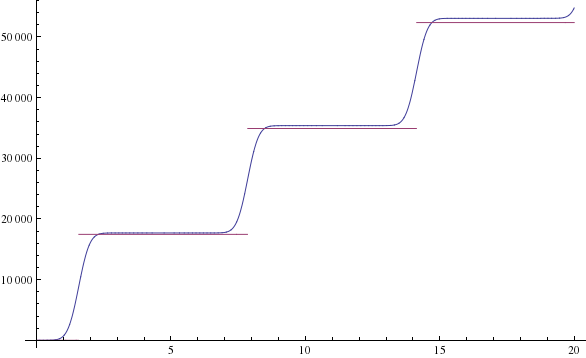
\includegraphics[width=0.5\columnwidth]{ladder.png}
\end{figure}

\noindent
Важно отметить, что реальное значение интеграла
такой функции по периоду отличается от апроксимации, полученной методом
перевала. При больших $x$, когда имеется вклад от большого количества
перевальных точек, эта погрешность складывается. Однако, относительная погрешность полученного результата по-прежнему остаётся малой.

\section*{Задача 3 (несколько перевалов)}

Найти асимптотическое поведение интеграла при $A\gg1$

\[
I(A)=\int_{-\infty}^{\infty}\exp(-A(x^{4}-x^{2}))dx
\]



\subsection*{Решение}

\begin{figure}[h]
	\caption{$y=x^{2}-x^{4}$}
	\centering
	\includegraphics[width=0.5\columnwidth]{lifshitz.eps}
\end{figure}

\noindent
Функция в показателе экспоненты имеет два максимума: 
\[
f^{\prime}(x)=0\Leftrightarrow4x^{3}-2x=0\Rightarrow x_{1,2}=\pm\frac{1}{\sqrt{2}}
\]

\noindent
Значения в перевальных точках определяются как:

\[
f(x_{1,2})=-A\left(\left(\pm\frac{1}{\sqrt{2}}\right)^{4}-\left(\pm\frac{1}{\sqrt{2}}\right)^{2}\right)\frac{A}{4}
\]

\noindent
А вторые производные:
\[
f^{\prime\prime}(x_{1,2})=-A(12x_{1,2}^{2}-2)=-4A
\]

\noindent
Поэтому в окрестности каждой из точек функция представляется как:
\[
f(x)\approx\frac{A}{4}-2A(x-x_{1,2})^{2}
\]

\noindent
Обе точки дадут вклад в перевальную оценку; поэтому для асимптотики
имеем:
\[
I\left(A\right)\approx\int_{-\infty}^{\infty}\exp\left(\frac{A}{4}-2A(x-x_{1})^{2}\right)dx+\int_{-\infty}^{\infty}\exp\left(\frac{A}{4}-2A(x-x_{2})^{2}\right)dx=\sqrt{\frac{2\pi}{A}}e^{A/4}
\]



\section*{Задача 4 (перевал $x^4$)}

Найти асимптотическое поведение интеграла при $A\gg1$:

\[
I\left(A\right)=\int_{-\infty}^{\infty}\exp\left(-A\left(\cosh x-\frac{x^{2}}{2}\right)\right)dx
\]



\subsection*{Решение}

Поскольку функция $\cosh x$ вблизи нуля раскладывается как $\cosh x\approx1+\frac{x^{2}}{2}+\frac{x^{4}}{24}+\dots$,
то видно, что ведущий член разложения функции в экспоненте имеет порядок
$x^{4}$. Поэтому, следуя идее метода перевала о разложении функции
в экспоненте в ряд около стационарной точки, для асимптотики этого
интеграла имеем:
\[
I(A)\approx\int_{-\infty}^{\infty}\exp\left(-A\left(1+\frac{x^{4}}{24}\right)\right)dx
\]

\noindent
Этот интеграл аналогичен интегралу Пуассона; его можно взять подстановкой
$t=\frac{A}{24}x^{4}$, сводящей его к гамма-функции:

\[
I(A)\approx e^{-A}\cdot2\int_{0}^{\infty}e^{-t}\left(\frac{24}{A}\right)^{1/4}\frac{1}{4}t^{-3/4}dt=\frac{1}{2}\left(\frac{24}{A}\right)^{1/4}e^{-A}\int_{0}^{\infty}t^{-3/4}e^{-t}dt=\left(\frac{3}{2A}\right)^{1/4}\Gamma\left(\frac{1}{4}\right)e^{-A}
\]

\noindent
Здесь $\Gamma\left(\frac{1}{4}\right)\approx3.62561$ --- просто некое
число; оно не выражается через известные мировые константы ($\pi$,
$e$, $C$, $\dots$); однако это и не требуется.

\section*{Задачи для домашнего решения}

\noindent \textbf{Упражнение 1}

\noindent Методом перевала приближенно вычислите интеграл при $\lambda\rightarrow+\infty$:
\begin{equation}
I(\lambda)=\int_{-1}^{1}\exp\left(\frac{\lambda}{\cosh^{2}x}\right)dx\text{.}	
\notag
\end{equation}

\vspace{15pt}
\noindent \textbf{Упражнение 2}

\noindent Методом перевала приближенно вычислите интеграл при $\lambda\rightarrow+\infty$:
\begin{equation}\notag
I(\lambda)	=\int_{0}^{+\infty}e^{-\lambda(x-1)^{2}(x-2)^{2}}dx.
\end{equation}

\vspace{15pt}
\noindent \textbf{Упражнение 3}

\noindent Методом перевала приближенно вычислите интеграл при $\lambda\rightarrow+\infty$:
\begin{equation}\notag
I(\lambda)=\int_{1}^{+\infty}\left(\frac{\ln x}{x}\right)^{\lambda}dx.	
\end{equation}

\vspace{15pt}
\noindent \textbf{Упражнение 4}

\noindent Используя идеи, аналогичные методу перевала, в пределе $\lambda\rightarrow+\infty$ вычислите интеграл
\begin{equation}\notag
I(\lambda)	=\int_{0}^{1}\exp(\lambda(\sin x-x)).
\end{equation}

\noindent \textit{Обратите внимание:} в перевальной точке вторая производная функции в показателе экспоненты равна 0.

\vspace{15pt}
\noindent \textbf{Задача 1}

\noindent В пределе $\lambda\rightarrow+\infty$ вычислите интеграл
\begin{equation}\notag
I(\lambda)	=\int_{-\infty}^{+\infty}e^{-x^{2}}\cosh^{\lambda}xdx.
\end{equation}

\vspace{15pt}
\noindent \textbf{Задача 2}

\noindent Рассмотрите интеграл с тремя параметрами:
\begin{equation}\notag
I(\lambda,\epsilon,s)	=\int_{0}^{+\infty}x^{s}e^{-\epsilon x}\exp(-\lambda(1-\cos x))dx.
\end{equation}

\noindent Вычислите его в пределе $\epsilon	\ll 1$, $\quad\lambda\gg1$,

\noindent считая, что $s$ - произвольное число порядка $1$.
\end{document}
